\documentclass[../paper.tex]{subfiles}

\begin{document}
  For the first prototype of our application the idea was to learn from
  previously done work and reuse what worked best. Additionally we followed
  general design principles like Gestalt laws \cite{wiki:principles_of_grouping}
  of grouping.

  A typical visualisation technique to make complex relationships clearly
  understandable is a graph layout. To show data flow from a data subject to one
  or more data processors, a graph works very well. Nodes represent data
  subject and data processors, and the links between them show that they relate
  with each other in such a way that data is shared between them. To make this
  even more clear, actual or imaginary data packets can be visualised as moving
  particles between the nodes. This feature makes it possible to give the
  visualisation a sense of directional flow.
  These design choices are also backed by Gestalt laws such as the law of
  similarity, which states that visual objects resembling each other are
  perceived as belonging to the same group. Further, the law of common fate
  states that objects moving into the same direction are recognised as grouped
  such as the data stream in the visualisation.

  \begin{figure}
    \centering
    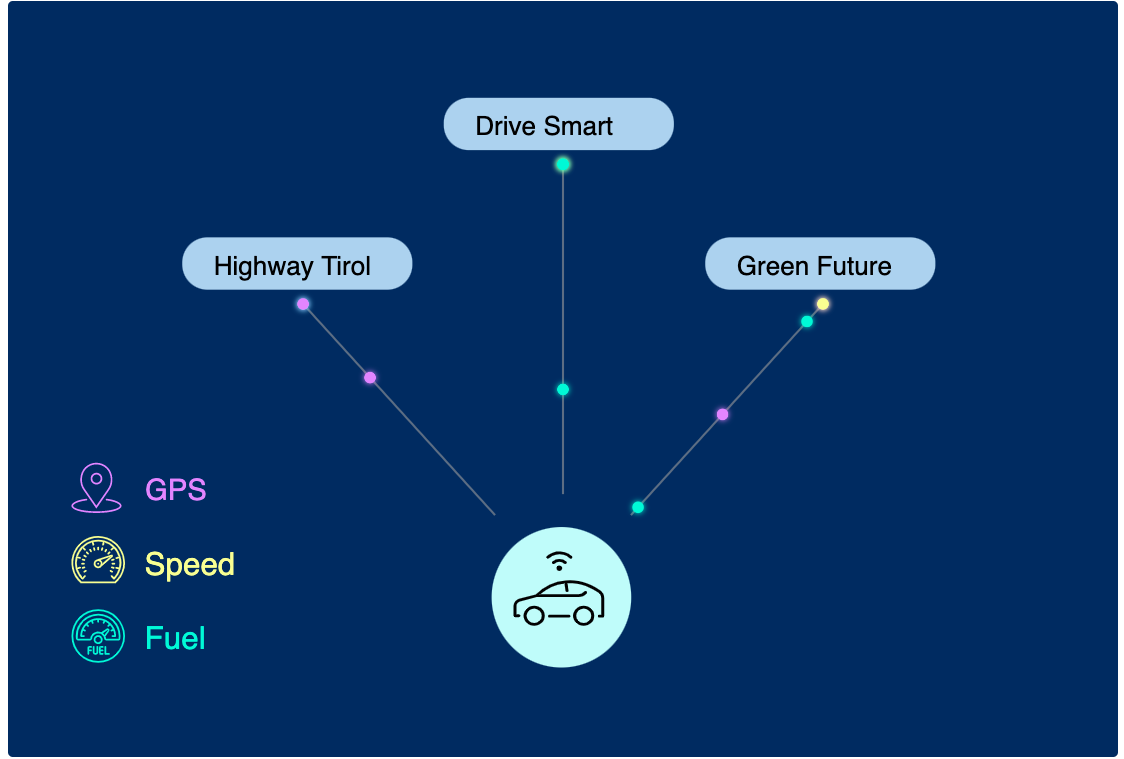
\includegraphics[width=\linewidth]{first-prototype}
    \caption{The first prototype of the general overview}
    \label{fig:prototype}
  \end{figure}

  Since the whole application is built around giving users a sense of control
  over their sharing activities, the user as a data subject stands in the centre of
  the visualisation with the connected data processors distributed around in a
  circle with the centre point
  being the user. Data processors, called campaigns in the CampaNeo environment, are
  represented by a rounded rectangle and the corresponding campaign name. The round
  particles represent data packets flowing from the user to the campaign. They are
  colour-coded to give additional information on the type of data that is sent,
  e.g. fuel consumption, speed or the GPS location of the car.
  The meaning of the different colours are encoded in a legend on the bottom left
  side of the screen. Here, words are paired with unambiguous symbols to make the
  legend easier and faster to read and understand. On the whole, the visualisation
  is designed to enable users to see at one glance what kind of data they are sharing
  and at what rate indicated by the data particle animation.

  With that we have now completely satisfied the defined needs of our application:
  The user can now find out with whom he shares what data and approximately at what
  rate. However, in case the user wants to get more in-depth information, it is
  possible to click on a specific data flow in the visualisation in order
  to get a more detailed view of the data stream. Here we rely on a time series
  visualisation and give additional information about the sensor that retrieved
  the data and the companies, with whom the data processor shares the collected data.

  Clarity is of utmost importance, which is why the visualisation always starts
  with the summary view to avoid confusing the user with too much information
  at once. The more detailed information is served only upon interacting with
  the visualisation. Displaying everything on screen at the same time would
  overload the initial rendering far too much. The moving particles, representing the
  data packets, are designed to directly draw a users attention on the centre of the
  application. Therefore, the animation of the flow is implemented as a loop, i.e.
  after the particles have arrived at their destination, they stay there for a short
  time before disappearing and flowing again from the centre.
\end{document}
